\section{Observation and Calculations}

We placed the two scintillation detectors are four different angles and took data for 3000s (15 mins.) each. The observations are summarised below. Figs. \ref{180}, \ref{170}, \ref{190}, \ref{90} show the \verb|CNSPEC| screenshots of the observational data. Part (a) of all the figures show the 3D heatmap of the peak counts against the channel numbers of both detectors on the x-y plane. 

\subsection{180$^\circ$}

\begin{figure}[H]
    % \ContinuedFloat
    \begin{subfigure}{\linewidth}
        \centering
        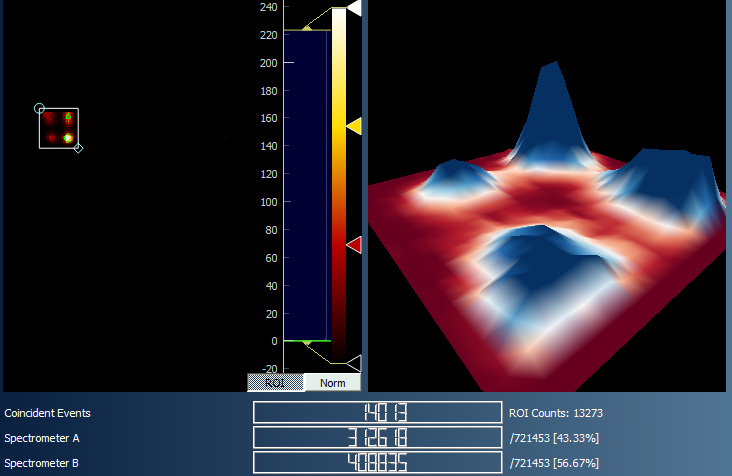
\includegraphics[width=1\textwidth]{images/180/3d.png}
        \caption{Coincidence plots: Heat map and 3D surface view}
    \end{subfigure}
    
    \bigskip
    \begin{subfigure}{\linewidth}
        \centering
        \includegraphics[width=0.9\textwidth]{images/180/calibration.png}
        \caption{Calibration of the 0.511 MeV photopeak}
    \end{subfigure}
    
    \bigskip
    \begin{subfigure}{\linewidth}
        \centering
        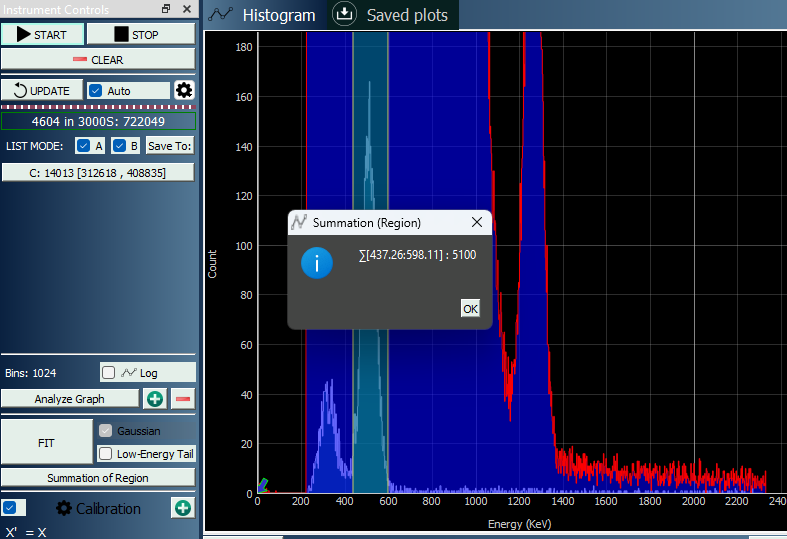
\includegraphics[width=1\textwidth]{images/180/ccred.png}
    \caption{Coincidence count of the red channel w.r.t. the blue channel = 5100}
    \end{subfigure}

    % \begin{subfigure}{\linewidth}
    %     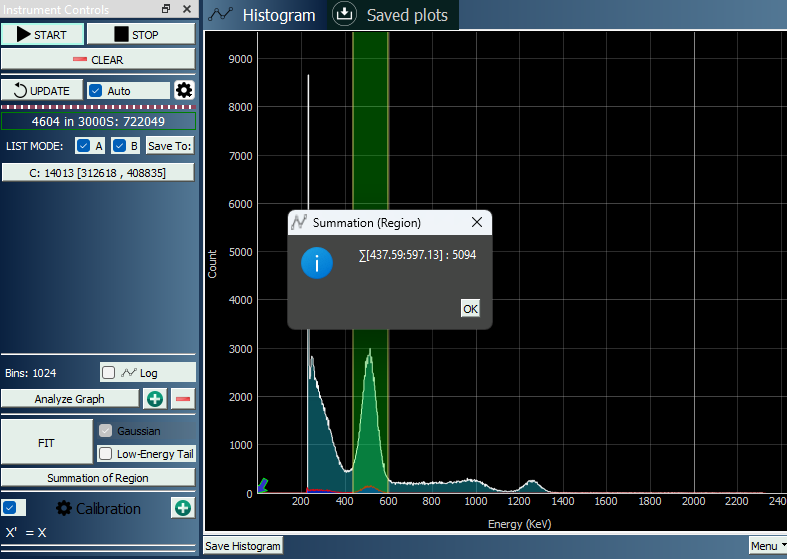
\includegraphics[width=1\textwidth]{images/180/ccblue.png}
    %     \caption{Coincidence count of the blue channel w.r.t. the red channel = 5094}
    % \end{subfigure}

    % \caption{\verb|CNSPEC| screenshots for $\gamma-\gamma$ coincidence with the detectors placed 180$^\circ$ to each other}
    % \label{180}
\end{figure}


\begin{figure}[H]
    \ContinuedFloat
    % % \bigskip
    % \begin{subfigure}{\linewidth}
    % 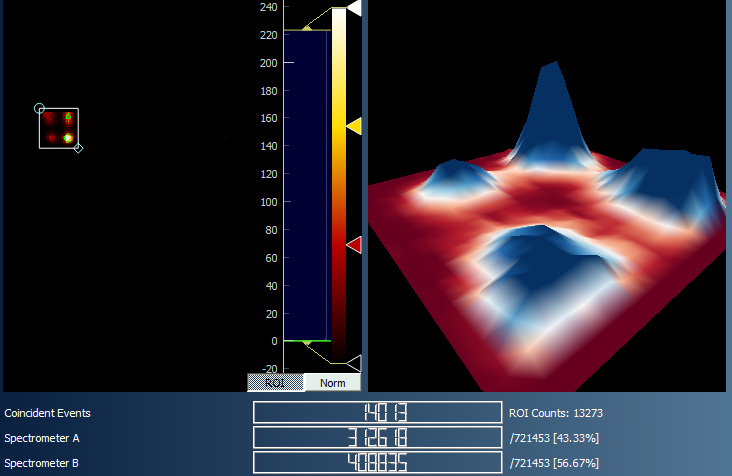
\includegraphics[width=1\textwidth]{images/180/3d.png}
    % \caption{Coincidence plots: Heat map and 3D surface view}
    % \end{subfigure}
    
    % \begin{subfigure}{\linewidth}
    %     \centering
    %     \includegraphics[width=0.7\textwidth]{images/180/calibration.png}
    %     \caption{Calibration of the 0.511 MeV photopeak}
    % \end{subfigure}
    
    % % \bigskip
    % \begin{subfigure}{\linewidth}
    %     \centering
    %     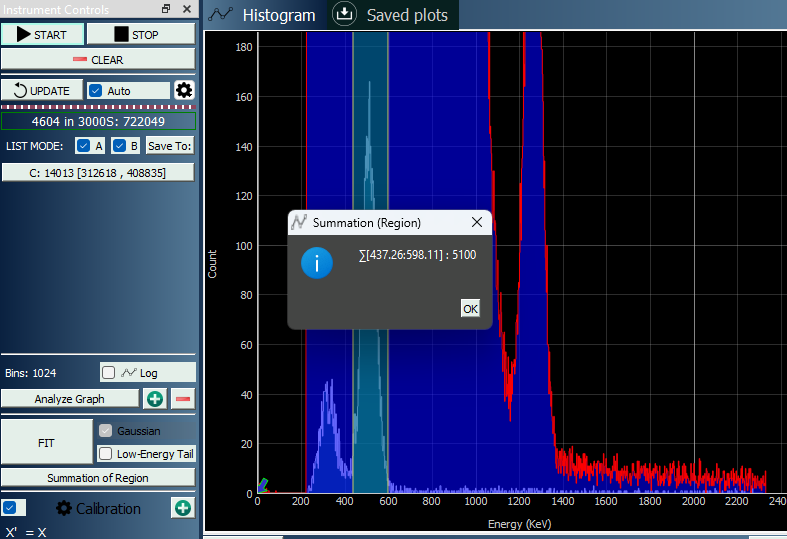
\includegraphics[width=1\textwidth]{images/180/ccred.png}
    % \caption{Coincidence count of the red channel w.r.t. the blue channel = 5100}
    % \end{subfigure}

    \begin{subfigure}{\linewidth}
        \centering
        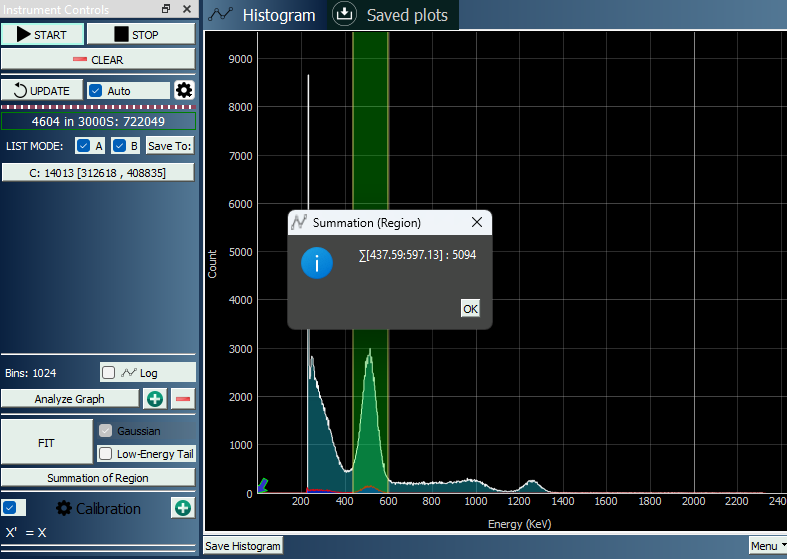
\includegraphics[width=1\textwidth]{images/180/ccblue.png}
        \caption{Coincidence count of the blue channel w.r.t. the red channel = 5094}
    \end{subfigure}

    \caption{CNSPEC screenshots for $\gamma-\gamma$ coincidence with the detectors placed 180$^\circ$ to each other}
    \label{180}
\end{figure}

\subsection{170$^\circ$}

\begin{figure}[H]
    % \ContinuedFloat
    % \bigskip
    \begin{subfigure}{\linewidth}
    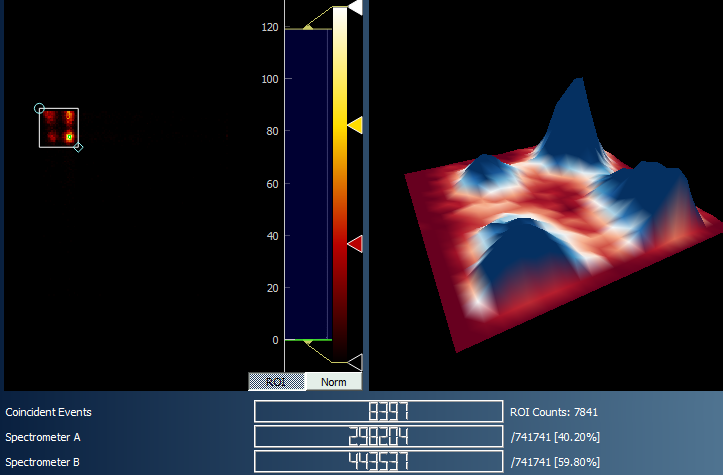
\includegraphics[width=1\textwidth]{images/170/3d.png}
    \caption{Coincidence plots: Heat map and 3D surface view}
    \end{subfigure}
    
    % \bigskip
    \begin{subfigure}{\linewidth}
    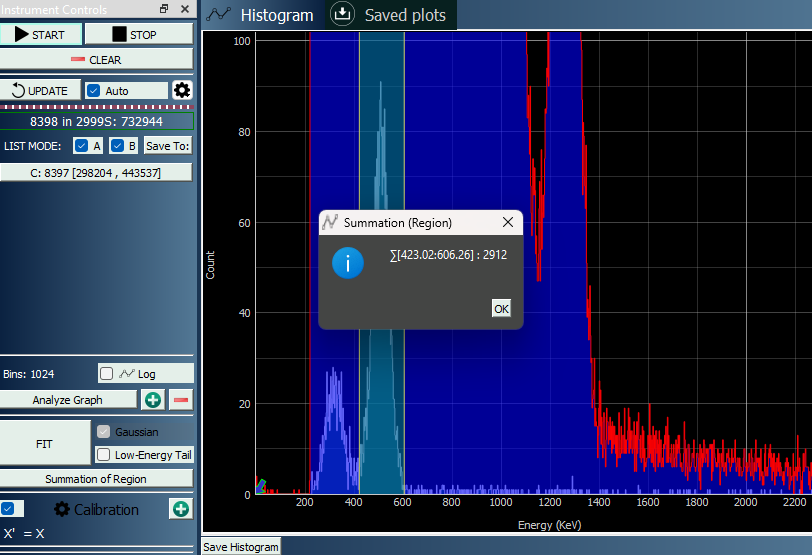
\includegraphics[width=1\textwidth]{images/170/ccred.png}
    \caption{Coincidence count of the red channel w.r.t. the blue channel = 2912}
    \end{subfigure}

    % \begin{subfigure}{\linewidth}
    %     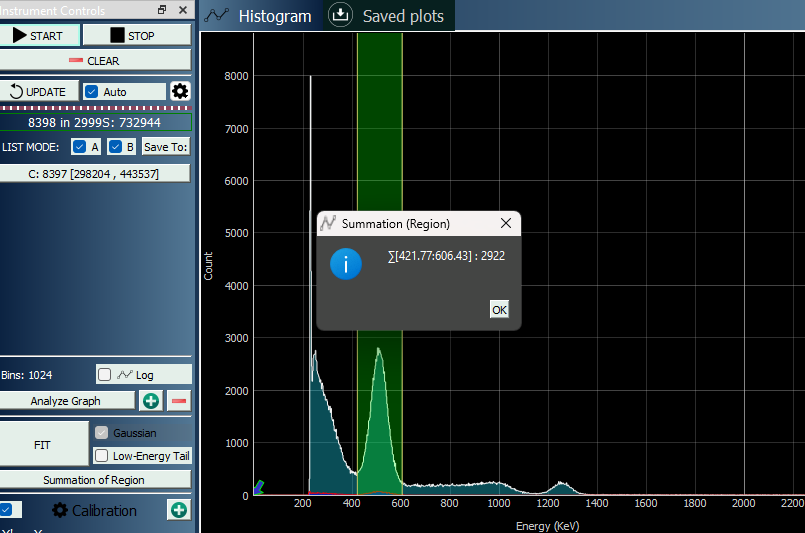
\includegraphics[width=1\textwidth]{images/170/ccblue.png}
    %     \caption{Coincidence count of the blue channel w.r.t. the red channel = 2922}
    % \end{subfigure}

    % \caption{CNSPEC screenshots for $\gamma-\gamma$ coincidence with the detectors placed 170$^\circ$ to each other}
    % \label{170}
\end{figure}

\begin{figure}[H]
    \ContinuedFloat
    % % \bigskip
    % \begin{subfigure}{\linewidth}
    % 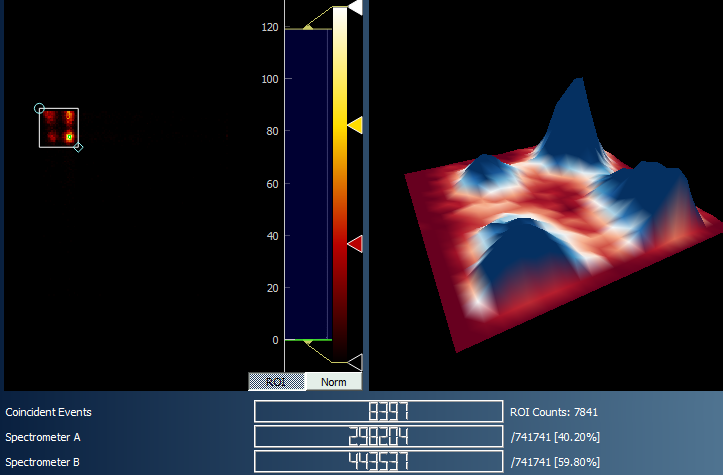
\includegraphics[width=1\textwidth]{images/170/3d.png}
    % \caption{Coincidence plots: Heat map and 3D surface view}
    % \end{subfigure}
    
    % % \bigskip
    % \begin{subfigure}{\linewidth}
    % 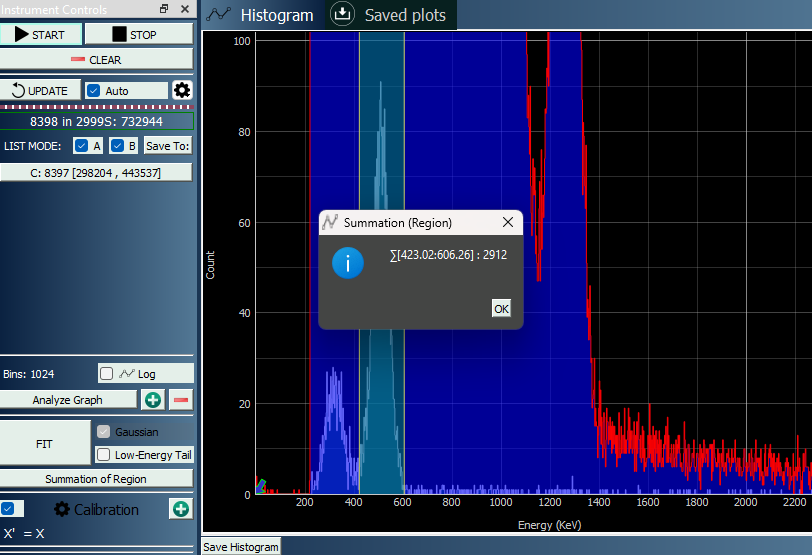
\includegraphics[width=1\textwidth]{images/170/ccred.png}
    % \caption{Coincidence count of the red channel w.r.t. the blue channel = 2912}
    % \end{subfigure}

    \begin{subfigure}{\linewidth}
        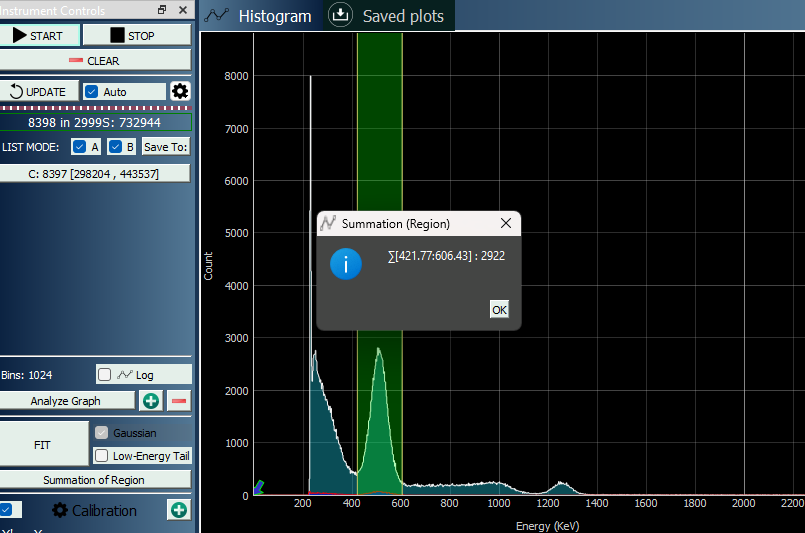
\includegraphics[width=1\textwidth]{images/170/ccblue.png}
        \caption{Coincidence count of the blue channel w.r.t. the red channel = 2922}
    \end{subfigure}

    \caption{CNSPEC screenshots for $\gamma-\gamma$ coincidence with the detectors placed 170$^\circ$ to each other}
    \label{170}
\end{figure}

\subsection{190$^\circ$}

\begin{figure}[H]
    % \ContinuedFloat
    % \bigskip
    \begin{subfigure}{\linewidth}
    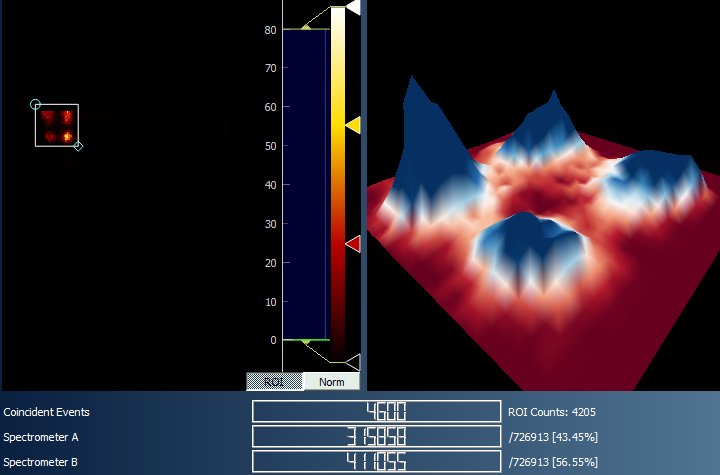
\includegraphics[width=1\textwidth]{images/190/3d.png}
    \caption{Coincidence plots: Heat map and 3D surface view}
    \end{subfigure}
    
    % \bigskip
    \begin{subfigure}{\linewidth}
    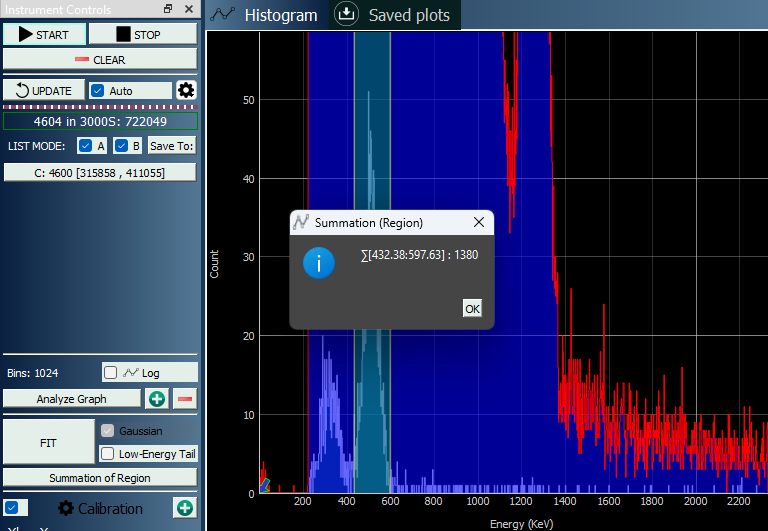
\includegraphics[width=1\textwidth]{images/190/ccred.png}
    \caption{Coincidence count of the red channel w.r.t. the blue channel = 1380}
    \end{subfigure}

    % \begin{subfigure}{\linewidth}
    %     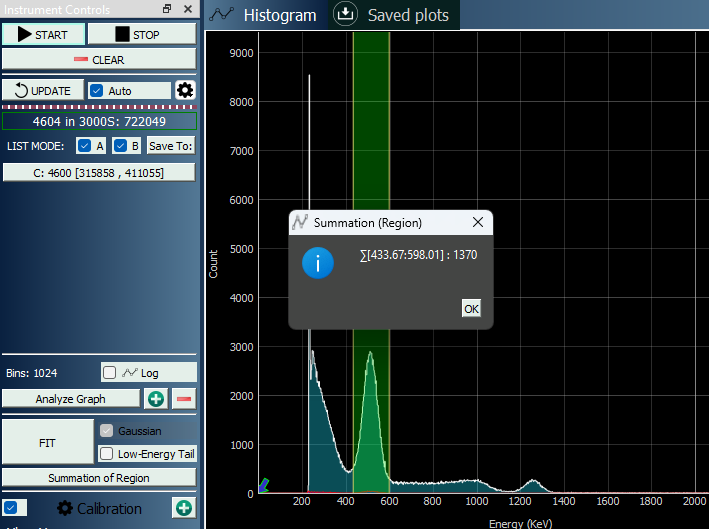
\includegraphics[width=1\textwidth]{images/190/ccblue.png}
    %     \caption{Coincidence count of the blue channel w.r.t. the red channel = 1370}
    % \end{subfigure}
    
    % \begin{subfigure}{\linewidth}
    %     \includegraphics[width=1\textwidth]{images/170/calibration.png}
    %     \caption{Calibration to 0.511 MeV photopeak}
    % \end{subfigure}

    % \caption{CNSPEC screenshots for $\gamma-\gamma$ coincidence with the detectors placed 190$^\circ$ to each other}
    % \label{190}
\end{figure}


\begin{figure}[H]
    \ContinuedFloat
    % \bigskip
    % \begin{subfigure}{\linewidth}
    % 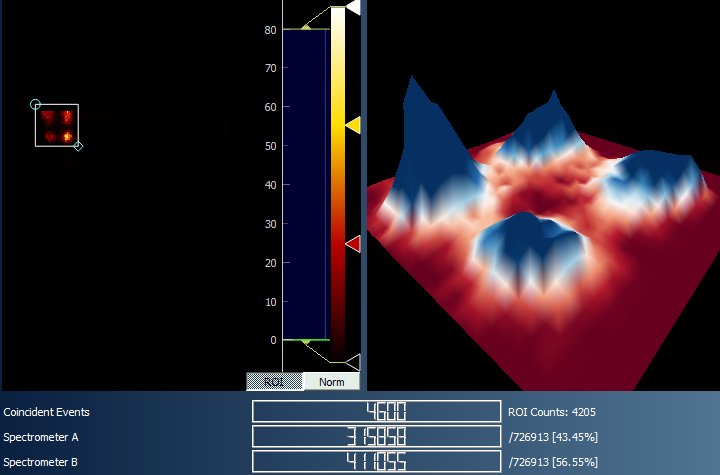
\includegraphics[width=1\textwidth]{images/190/3d.png}
    % \caption{Coincidence plots: Heat map and 3D surface view}
    % \end{subfigure}
    
    % % \bigskip
    % \begin{subfigure}{\linewidth}
    % 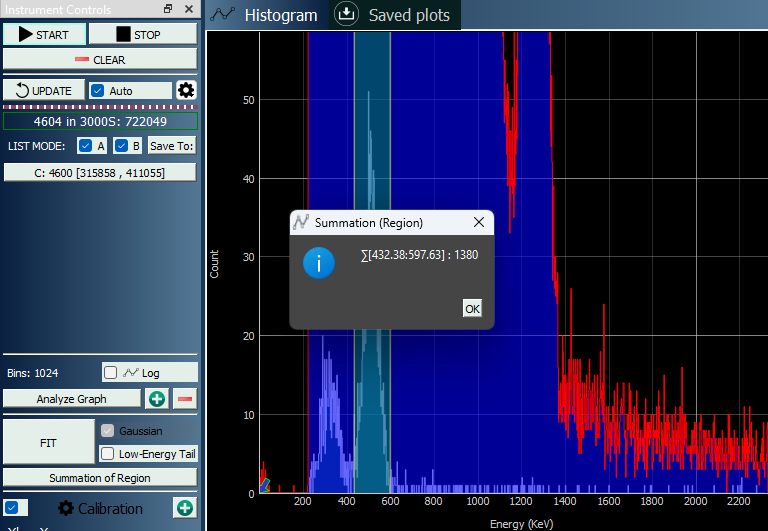
\includegraphics[width=1\textwidth]{images/190/ccred.png}
    % \caption{Coincidence count of the red channel w.r.t. the blue channel = 1380}
    % \end{subfigure}

    \begin{subfigure}{\linewidth}
        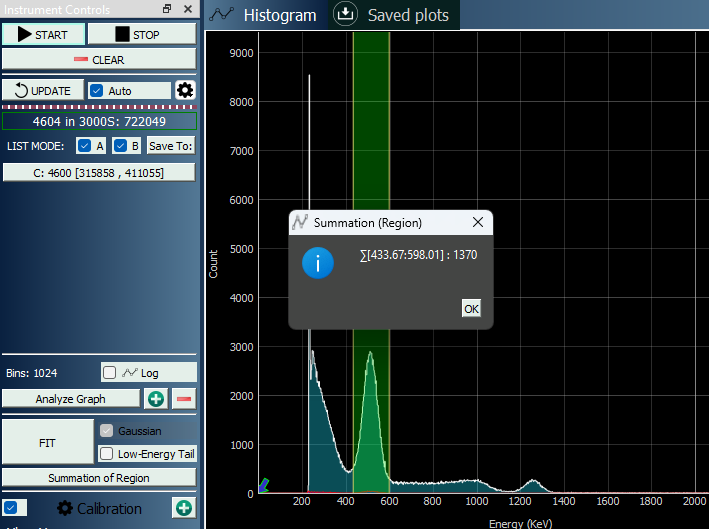
\includegraphics[width=1\textwidth]{images/190/ccblue.png}
        \caption{Coincidence count of the blue channel w.r.t. the red channel = 1370}
    \end{subfigure}
    
    \caption{CNSPEC screenshots for $\gamma-\gamma$ coincidence with the detectors placed 190$^\circ$ to each other}
    \label{190}
\end{figure}

\subsection{90$^\circ$}

\begin{figure}[H]
    % \ContinuedFloat
    % \bigskip
    \begin{subfigure}{\linewidth}
    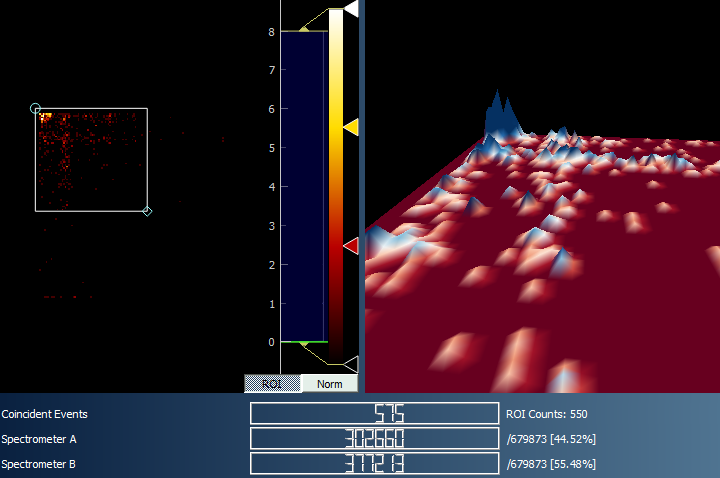
\includegraphics[width=1\textwidth]{images/90/3d.png}
    \caption{Coincidence plots: Heat map and 3D surface view}
    \end{subfigure}
    
    % \bigskip
    \begin{subfigure}{\linewidth}
    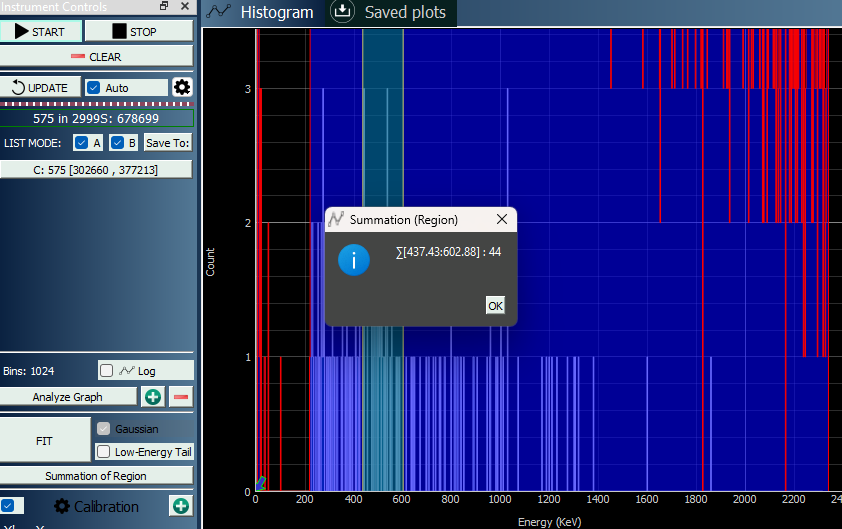
\includegraphics[width=1\textwidth]{images/90/ccred.png}
    \caption{Coincidence count of the red channel w.r.t. the blue channel = 44}
    \end{subfigure}

    % \begin{subfigure}{\linewidth}
    %     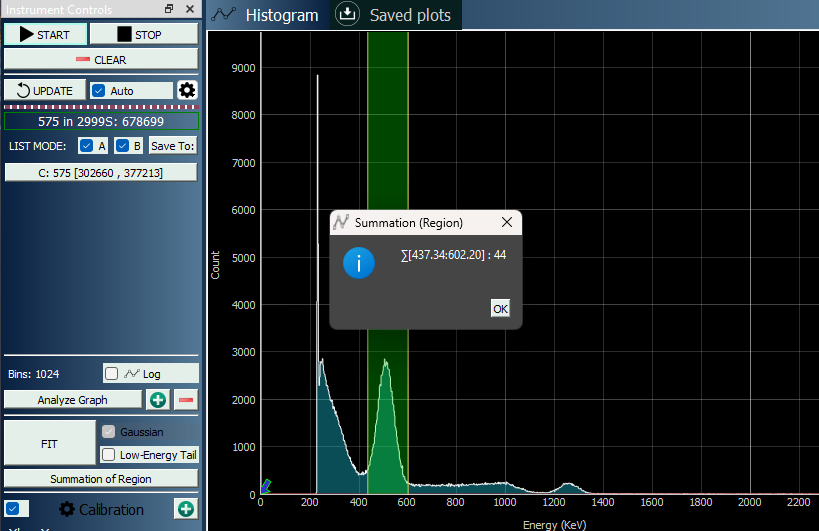
\includegraphics[width=1\textwidth]{images/90/ccblue.png}
    %     \caption{Coincidence count of the red channel w.r.t. the blue channel = 44}
    % \end{subfigure}
    
    % \begin{subfigure}{\linewidth}
    %     \includegraphics[width=1\textwidth]{images/170/calibration.png}
    %     \caption{Calibration to 0.511 MeV photopeak}
    % \end{subfigure}

    % \caption{CNSPEC screenshots for $\gamma-\gamma$ coincidence with the detectors placed 90$^\circ$ to each other}
    % \label{90}
\end{figure}


\begin{figure}[H]
    \ContinuedFloat
    % \bigskip
    % \begin{subfigure}{\linewidth}
    % 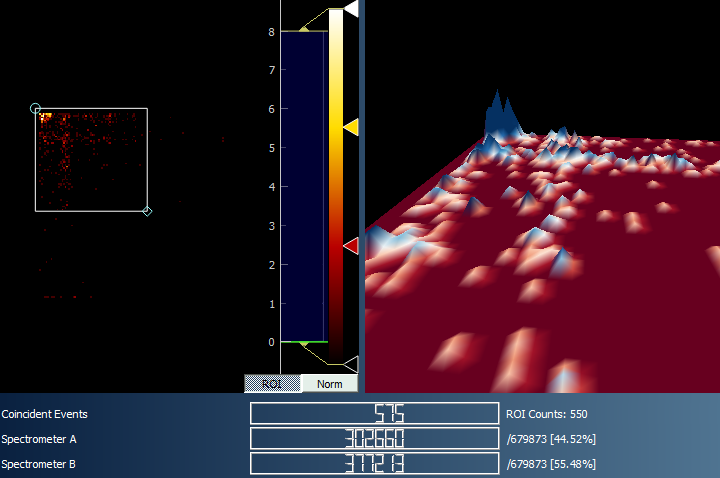
\includegraphics[width=1\textwidth]{images/90/3d.png}
    % \caption{Coincidence plots: Heat map and 3D surface view}
    % \end{subfigure}
    
    % % \bigskip
    % \begin{subfigure}{\linewidth}
    % 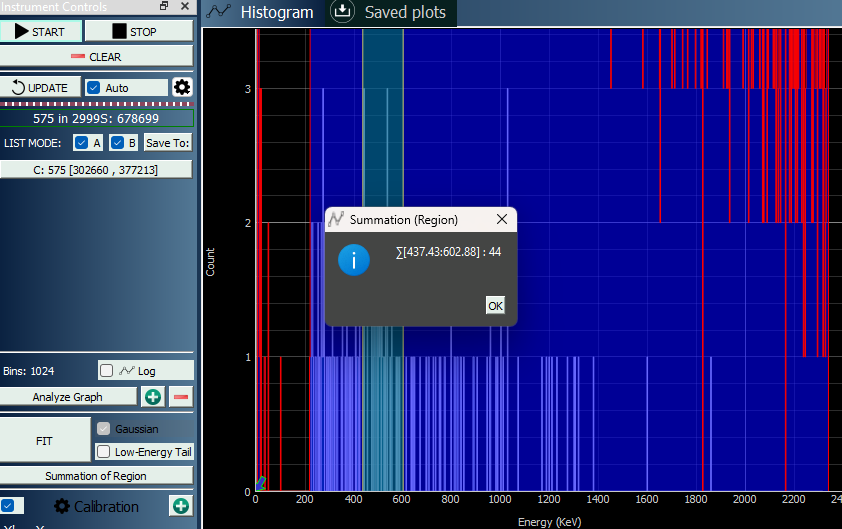
\includegraphics[width=1\textwidth]{images/90/ccred.png}
    % \caption{Coincidence count of the red channel w.r.t. the blue channel = 44}
    % \end{subfigure}

    \begin{subfigure}{\linewidth}
        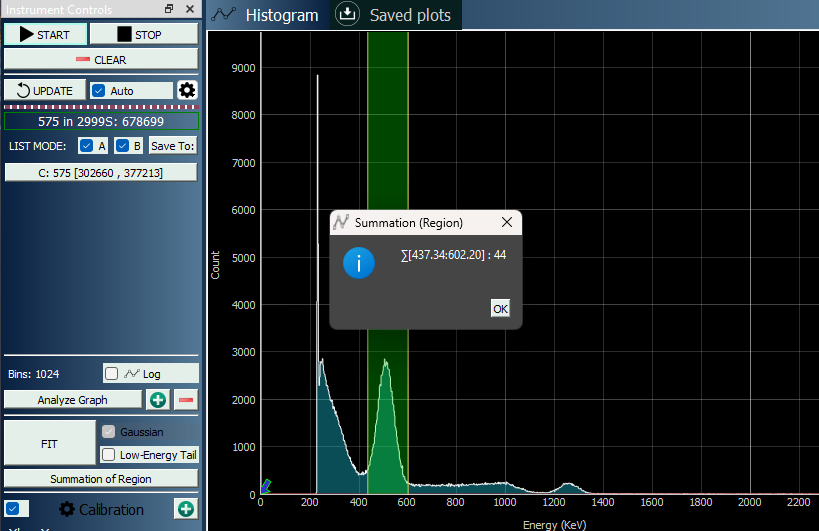
\includegraphics[width=1\textwidth]{images/90/ccblue.png}
        \caption{Coincidence count of the red channel w.r.t. the blue channel = 44}
    \end{subfigure}
    
    % \begin{subfigure}{\linewidth}
    %     \includegraphics[width=1\textwidth]{images/170/calibration.png}
    %     \caption{Calibration to 0.511 MeV photopeak}
    % \end{subfigure}

    \caption{CNSPEC screenshots for $\gamma-\gamma$ coincidence with the detectors placed 90$^\circ$ to each other}
    \label{90}
\end{figure}

The average coincidence counts for each angle in 15 minutes is:

\begin{itemize}
    \item for 90$^\circ$: 44 counts
    \item for 170$^\circ$: 2917 counts
    \item for 180$^\circ$: 5097 counts
    \item for 190$^\circ$: 1375 counts\\
\end{itemize}

The count rates are plotted against their corresponding angles in Fig. \ref{plt}.

\begin{figure}[H]
    \centering
    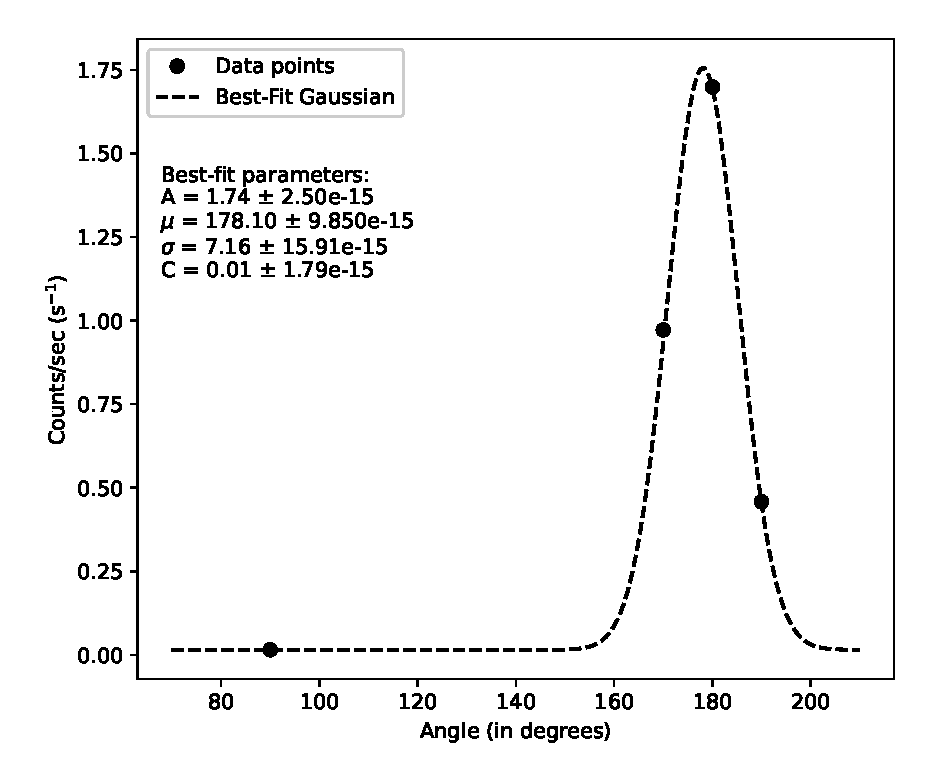
\includegraphics[width=1\columnwidth]{images/plt.eps}
    \caption{Count rates vs. angle plot}
    \label{plt}
\end{figure}